\documentclass[a4paper, two column]{article}

\usepackage[utf8]{inputenc}
\usepackage{multicol}
\usepackage{amsmath}
\usepackage{amsfonts}
\usepackage{tikz}
\usepackage{graphicx}
\usepackage{mdframed}
\usepackage{color}
\usepackage{listing}
\usepackage{wrapfig}
\usepackage[parfill]{parskip}
\usepackage{subcaption}
\usepackage{hyperref}
\usepackage[font={footnotesize}]{caption}
\usepackage{marvosym}
\usepackage[margin=0.7in]{geometry}
\usepackage{tablefootnote}
\usepackage{abstract}
\usepackage{enumerate}
    \makeatletter
    \let\@fnsymbol\@arabic
    \makeatother
\begin{document}
\twocolumn[{
\centering
{\LARGE \textbf{GPU-accelerated facet-based convolutional gridding}}\\
{\large \textbf{The problem of non-coplanar widefield imaging in radio astronomy}}\\
Benjamin Hugo\thanks{bennahugo@aol.com}\\
Supervised by: A/Prof. James Gain\thanks{jgain@cs.uct.ac.za} and Prof. Oleg Smirnov\thanks{o.smirnov@ru.ac.za}\\[0.5cm]
}]
\saythanks
\section{Context}
Modern radio astronomy observes electromagnetic emissions with wavelengths typically around one million times longer than that of visible light, and astronomers are subsequently 
able to observe phenomena that are scattered by the interstellar medium, at the wavelengths of visible light. Since its birth in the early 20th century, research has been largely 
driven towards building telescopes with higher resolving capability. In modern radio astronomy this is achieved through aperture synthesis, which combines the resolving capacity 
of smaller apertures to provide an equivalent resolving capability to that of a single, much larger aperture \cite{christiansenradiotelescopes}.

In imaging mode the goal is to densely sample these electromagnetic wavefronts (assumed planar when arriving at the antennae) in a local coordinate framework, and through inversion 
determine the intensities of the emitting sources. These intensities are visualized as an ``image'' of the sky. The image is assumed to be a small region on a unit sphere, with no 
contributing emission sources within the sphere. Refer to figure~\ref{FIG_APERTURE_SYNTH}.

\begin{figure}[h]
 \begin{mdframed}
 \centering
 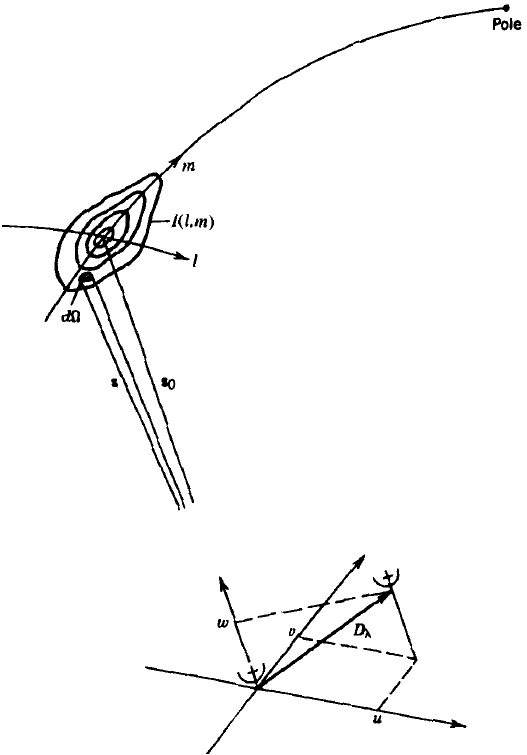
\includegraphics[width=0.7\textwidth]{lmn_uvw.png}
 \caption[The relation between image space and visibilities]{The relation between the sampled local coordinate frame (u,v,w space) and the projected source on the unit ``celestial'' 
 sphere (l,m,n space). The telescope points at a pointing centre $s_0$. The lmn coordinates are the direction cosines describing the positions of sources on the unit sphere. The electromagnetic radiation
 of these sources are assumed to arrive as planar wavefronts at the antennae. Image courtesy of Thompson et al. \cite{thompson2008interferometry}.}
  \label{FIG_APERTURE_SYNTH}
 \end{mdframed}
\end{figure}

Obviously it will be impractical to construct an array of antennae to completely sample this local coordinate frame in a single instant. Instead, as the earth slowly rotates, the 
relative direction between pairs of antenna sweeps out elliptical paths through the local coordinate space. Provided that the observation is long enough (usually made over several hours), 
and that the antennae keep pointing towards the same position in the sky, enough of the electromagnetic interference can be collected to distinguish even faint sources from 
background noise. See figure~\ref{FIG_IMAGE_FORMATION}.

\begin{figure}[h]
 \begin{mdframed}
  \begin{subfigure}[b]{\textwidth}
   \centering
   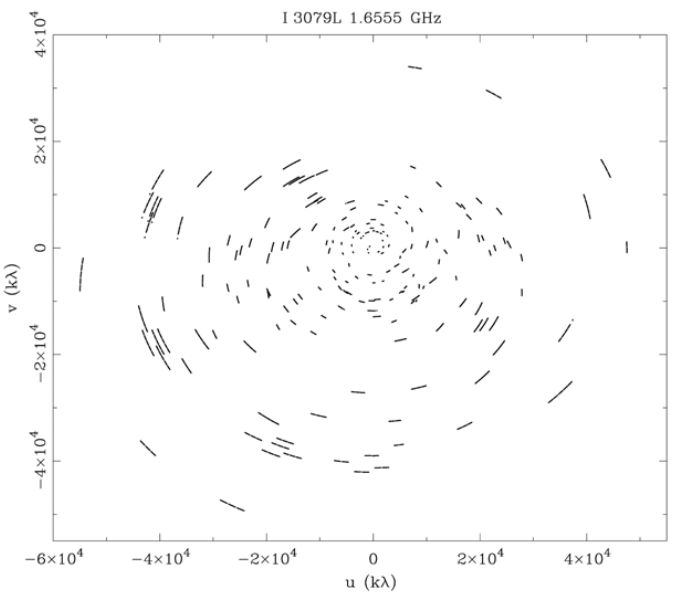
\includegraphics[width=0.5\textwidth]{uv_space.png}
   \caption{}
   \label{FIG_IMAGE_FORMATION_A}
  \end{subfigure}
  \begin{subfigure}[b]{\textwidth}
   \centering
   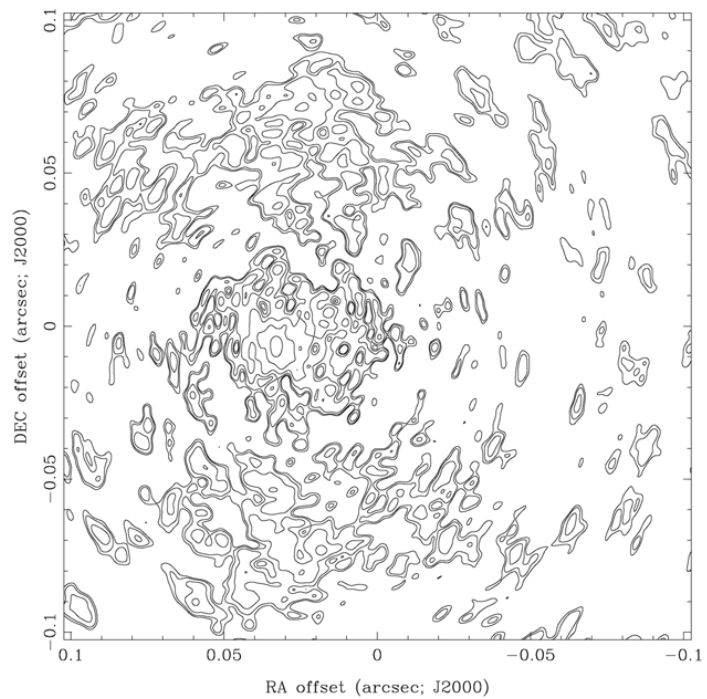
\includegraphics[width=0.5\textwidth]{lm_space.png}
   \caption{}
   \label{FIG_IMAGE_FORMATION_B}
  \end{subfigure}
  \caption[Sampled uv space and its image]{\ref{FIG_IMAGE_FORMATION_A} shows the elliptically sampled local coordinate frame (uv coordinates), while \ref{FIG_IMAGE_FORMATION_B} shows the 
					   unprocessed, ``dirty'' image formed by the inversion process. Images courtesy of Middelberg et al. \cite{middelberg2008high}}
  \label{FIG_IMAGE_FORMATION}
 \end{mdframed}
\end{figure}

That said, in reality the space is only densely sampled around the origin, see figure~\ref{FIG_PSF}, and only a single plane is usually considered when inverting the samples to an image. This 
requires all the direction vectors (or ``baselines'') between pairs of antennae to stay on the same plane for the duration of an observation. However, to observe the sky at lower declinations 
(at an angle close to the horizon), arrays with elements both parallel and perpendicular to the rotation of the earth must be used. The baselines of these two-dimensional arrays do not remain 
planar over the duration of a single observation and cause image distortions. 

\begin{figure}[h]
 \begin{mdframed}
 \centering
 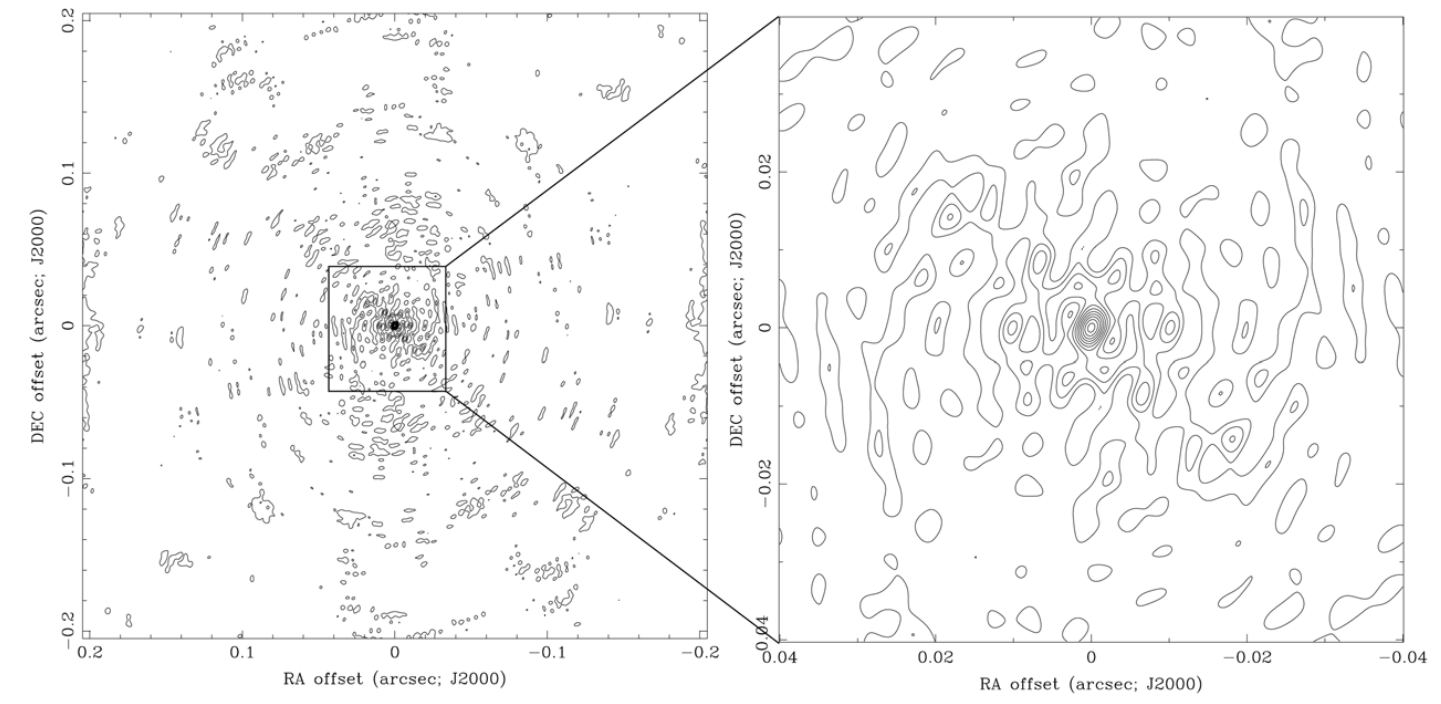
\includegraphics[width=1.0\textwidth]{psf.png}
 \caption[PSF]{Sampled regions of the same image shown in figure~\ref{FIG_IMAGE_FORMATION}. Areas further away from the pointing centre are not densely sampled, and require further processing to form a
 ``clean'' image. Image courtesy of Middelberg et al. \cite{middelberg2008high}.}
  \label{FIG_PSF}
 \end{mdframed}
\end{figure}

To add to this problem of non-coplanar baselines, the computational complexity of the inversion process requires that areas on the unit celestial sphere be approximated by a flat plane. This 
plane approximation to the celestial sphere is only valid in a small area around the tangent point (the pointing centre of the telescope). When imaging wider fields of views the curvature of the sky
can no longer be ignored. Under these conditions the distortions caused by non-coplanar baselines are intensified and other techniques must be employed to remove these effects. These techniques are
reasonably expensive, both in terms of extra memory and computational requirements, which makes the already-expensive synthesis process even more costly. Collectively the problem is known as the 
\textit{problem of non-coplanar widefield imaging} \cite{taylor1999synthesis}. 

This forms the problem context of our research. The exact details of the inversion process, corrective techniques, research process, as well as a short literature survey will be discussed next.

\section{Methodology}
\subsection{Widefield imaging algorithms}
The inversion process mentioned earlier refers to the inversion of the fourier relation between the sampling and imaging spaces. Each antenna measures the contribution from each source (its intensity) as the cosine 
between the pointing direction and source direction. Refer back to figure~\ref{FIG_APERTURE_SYNTH}. To measure most of the incoming energy the signal integration between pairs of antennae alluded to earlier measures two voltages: a cosine 
with no phase offset and a cosine with a phase offset (or equivalently a signal delay) of 90 degrees - a sine term. Each visibility sample in the local antenna coordinate frame is expressed as a sum of cosine and sine 
contributions from multiple sources (a fourier series) \cite{taylor1999synthesis}.

There are very fast algorithms for taking the inverse fourier transform (Cooley-Tukey for instance), but they require that the visibilies are sampled at regular intervals. This is not true of real observations. 
To overcome this issue the visibilities (per baseline, time step and observed frequency channel) are resampled onto a regular grid by ``interpolating'' each visibility onto, possibly, multiple grid cells. This is done by 
multiplying each visiblity term with a precomputed, oversampled, function (such as the one described by Sze Tan \cite{tan1986aperture}) and adding these values back onto the grid. This process is known as \textit{convolutional gridding}. The inverse process known as 
\textit{convolutional degridding} attempts to predict the original sampled visibilities by summing over the weighted grid cells (the opposite of the gridding process) \cite{taylor1999synthesis}.

The other, more accurate, approach to doing the inversion which does not require doing convolutional gridding, is to compute the intensity of each pixel directly (a sum over all the visibility terms). This approach is infeasible
(complexity of O($N^4$) and a memory requirement of up to O($N^3$) when taking non-coplanar widefield imaging corrections into account). Convolutional gridding has a complexity 
of roughly O($N^2\log_2{N}$) + O($N^2C^2$), where $C^2$ is the number of cells in the precomputed gridding function, and is the preferred imaging method \cite[Lecture 7]{taylor1999synthesis}.

Both convolutional gridding and its inverse, convolutional degridding, can be parallelized and are suitable for processing on massively multicore architectures such as General Purpose GPUs. Although convolutional gridding 
has been implemented on GPUs in past research (for example \cite{romein2012efficient}), the grid sizes required by the Square Kilometer Array ($10^{10}$ pixels \cite{cornwell2012wide}) cannot be fitted in the onboard memory 
of current GPU accelerators. This problem can be mittigated by facet-based imaging, where each image is split into multiple smaller facets, and synthesized independently of eachother. 

This image-space faceting approach involves dividing the celestial sphere into small approximating planes (in other words the sphere is approximated by a polyhedron). This is achived by phase rotating each visibility
towards the centre of each computed facet, as well as rotating the local uvw coordinate frame in order to ensure that each facet image is tangent to the celestial sphere \cite{cornwell1992radio}. In coplanar faceting
the latter coordinate transformation is not computed \cite{AIPS113}.

Faceting, along with the methods of w-projection (applying a w-dependent corrective convolution function \cite{cornwell2005w}) or snapshots (a series of short-time observations over which the baselines are assumed to be coplanar) will 
also eliminate the distortions caused by imaging wider fields of view discussed earlier. See figure~\ref{FIG_3D_DISTORTIONS} for an illustration of these distortions and the 
results of applying corrective faceting and w-projection.

\begin{figure}[h]
 \begin{mdframed}
 \centering
 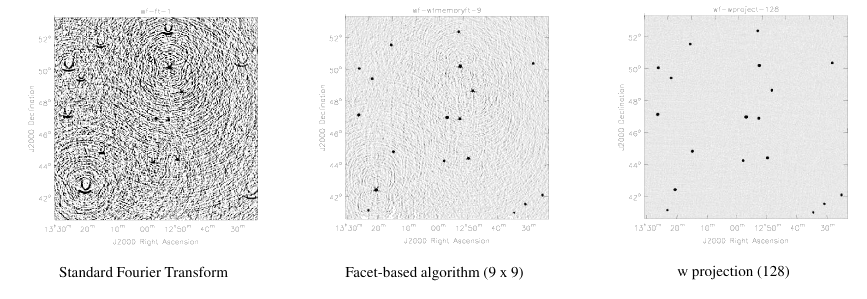
\includegraphics[width=0.5\textwidth]{3d_correction.png}
 \caption{The distortions caused by widefield imaging without corrections (standard Fourier transform) and with 3D corrections (faceting and w-projection). Image by Cornwell et al. \cite{1416440}}
  \label{FIG_3D_DISTORTIONS}
 \end{mdframed}
\end{figure}

Although computing a fully faceted image is considered to be an order of magnitude slower (in seconds) than w-projection \cite{1416440}, it has significantly reduced memory requirements when compared 
to doing w-projection-based convolutional gridding, computing each voxel in a direct transform approach or separately gridding each w-plane before taking a three-dimensional fourier 
transform \cite{yashar2009tdp}. For this reason we opt to support a targeted faceting approach, where facets are only computed over relatively few areas of interest. 
See figure~\ref{IMG_PERFORMANCE_COMPARISON} for a comparative plot.
\begin{figure}
 \begin{mdframed}
  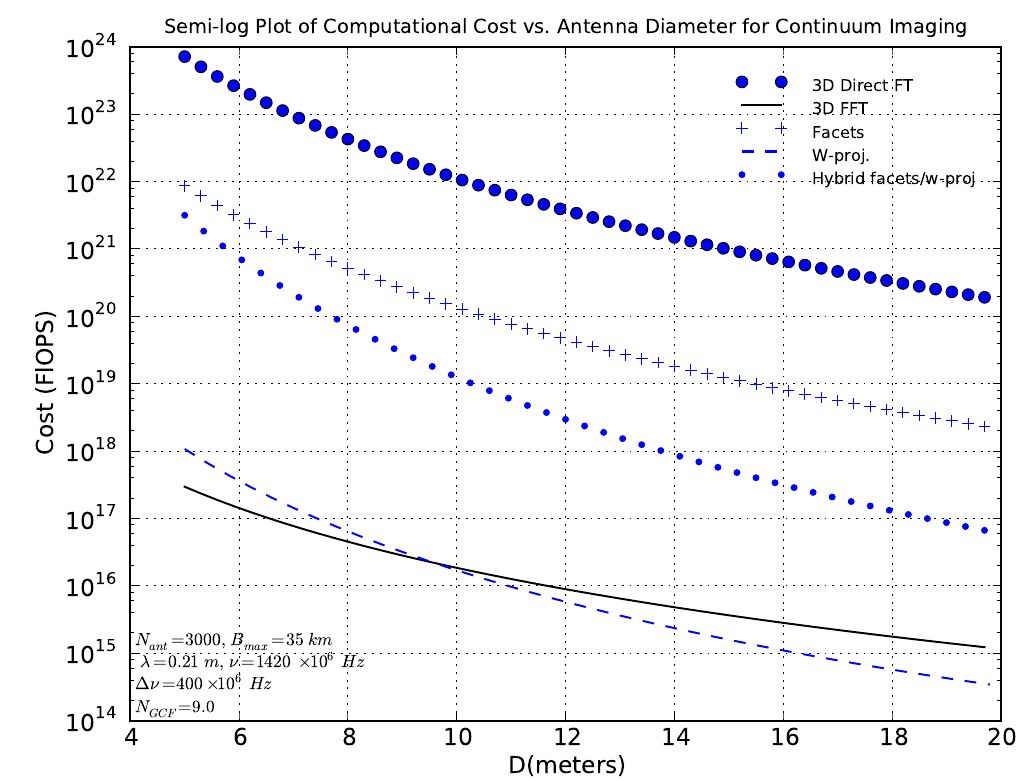
\includegraphics[width=1.0\textwidth]{performance_faceting.png}
  \caption{Plots of computational cost (floating point operations per second vs. antenna diameter D) of several schemes including w-projection and hybrid faceting and w-projection. Taken from an analysis by Yashar and Kemball \cite{yashar2009tdp}.}
  \label{IMG_PERFORMANCE_COMPARISON}
 \end{mdframed}
\end{figure}

When performing targeted faceting it is not, in general, required to recombine the different facets back into a single image, since most of the image will be empty. A fully faceted image, however 
requires reprojecting the individual facets onto a single plane. This projection \cite{sault1996approach} is well documented and has already been implemented in several packages, including 
the AIPS task ``FLATN'' \cite{AIPS113}.

Lastly, our implementation will make provision for correcting the time-invariant (or slowly variant) directionally dependent effects on the observed visibility samples. 
These slow-varying directional dependent effects, such as those introduced by the ionosphere and antenna beam patterns are locally invariant, and can subsequently be approximated and corrected for 
individual facets (provided these facets are small enough) \cite{2011A&A...527A.106S,2011A&A...527A.107S}.

\subsection{Objectives}
The focus of our research is not on generating new methods of imaging, but merely accelerating the widely known and used method of facet-based synthesis imaging. The novelty of the research undertaken 
lies solely in the acceleration of a known algorithm. To the best of our understanding the problem is suitable for GPU acceleration, and our research simply aims to explore this approach to imaging 
as a viable solution to the memory requirement constraints of current techniques.

Our research aims to achieve the following key objectives, in 3 distinct phases:
\begin{enumerate}[i)]
 \item \textbf{Implement an optimized CPU-based faceted convolutional gridder in C++}\\
  A multi-core implementation will be constructed using OpenMP and AVX vector intrinsics, where applicable. It will serve as a reasonable baseline for performance 
  comparisons of a GPU-based version and previous research. The imager will make provision for both image and uv space faceting, as well as targetted and full-image faceting. It will 
  additionally provide facilities to load correcting terms (per antenna and direction) as discussed earlier. This phase of the research is already underway.
 \item \textbf{Implement a GPU-based faceted convolutional grider in CUDA}\\
  The GPU version will be based on the most work-efficient GPU gridding algorithm in the literature, but will be modified to include faceting instead of w-projection. This version
  can be numerically checked for accuracy and the optimizations benchmarked against the CPU version implemented earlier.
 \item \textbf{Create a distributed solution using the Message Passing Interface}\\
  The sheer scales of these tasks ensures that both a purely parallel CPU version and a GPU version of the faceted gridder can benefit from additional computing power offered by even that of a small cluster.
\end{enumerate}

We will consider the project successful if the distributed GPU imager is substantially faster (40-50x) compared to (optimized) CPU-based faceted imaging. We will discuss several performance metrics next.

\subsection{Performance metrics}
Previous gridding literature \cite{muscat2014high,romein2012efficient} has made comparisons in terms of ``Gigagridpoint additions per second'' and we will measure the same performance metric in order to judge 
whether the gridder is on par with those described in the literature. The measure of throughput (size of input visibilities / total seconds to grid facets) can be used to judge how well the implementation is 
using available GPU memory bandwidth (which is typically more than an order of magnitude slower than the floating point processing capability of modern GPUs). This assumes the processing time computing each 
facet significantly outweighs the cost of transferring memory to and from the GPU.

Throughput will likely be one of the most important performance metrics and may be more pertinent for measuring gridding performance on GPUs when compared to measuring performance 
as floating point operations per second. The reason is that the the performance of convolutional gridding can be considered to be a memory bound problem. Typically each global memory access may take hundreds of 
clock cycles, compared to only a few clock cycles per arithmetic operation. Arithmetic intensity (number of operations performed per byte accessed in memory \cite{sclocco2014auto}) gives a good estimation of 
whether the algorithm will be compute or memory bound. To obtain good GPU performance the arithmetic intensity has to be high. Convolutional gridding does not involve a significant amount of arithmetic per 
global memory access, and can therefore not exploit the peak computational capability of a GPU. Although faceting adds additional complex exponentiations and coordinate transformations to each visibility, it 
also adds additional memory accesses. We believe that faceting will not substantially alter the arithmetic intensity and the problem will remain memory bound.

Substantial parallelization may translate to speedups which can mean the difference between hours and possibly minutes of computation time for a single image. Targeted faceting over sparse images (described earlier) will
be the optimal situation for using an accelerated faceting approach, since this will significantly reduce the amount of computation time involved with creating an image. 

\subsection{Data sources}
Obtaining real observation data and reading these datasets for performance benchmarking will not be a problem. We have access to real observation data 
from the KAT-7 telescope, as well as well-tested and documented third party libraries which can read and convert between popular formats. 

It is also possible to generate a large synthetic dataset with several point sources, using the uv sampling coordinates of a real telescope such as LOFAR or KAT-7 in order to 
test the output of the faceted gridder.

\subsection{Validity}
To ensure that the images produced by our gridder are correct they will be compared to the dirty images produced by well-known radio imaging toolsets which supports three-dimensional correction techniques (ie. w-projection or faceting). Faceting has
for instance been the defacto standard in the Astronomical Image Processing System (AIPS) task ``IMAGR'' \cite{AIPS113} and is also supported in newer toolkits such as the Common Astronomy Software Applications (CASA) \footnote{Freely available from \url{casa.nrao.edu}}. 
The latter, along with other well-known tools, such as the MeqTrees imager ``Tigger'' can be used for validation purposes.

\subsection{Resources required} 
This project will not require substantial resources beyond the use of the UCT High Performance HEX cluster (or possibly the cluster at the Center for High Performance Computing). It may be possible to also benchmark the algorithm performance
on newer hardware such as the Tesla K10 on the Amazon EC cloud for a small hourly fee (\$0.650 USD \footnote{Available from \url{http://aws.amazon.com/ec2/pricing/}. This is the quoted price at the time of writing (15 June 2014, 17:37).}). For development purposes we have 
access to a Nvidia GeForce GTX 770 and a 4th generation Intel i7 CPU with support for the AVX 2.0 instruction set. This research will not require any ethical clearance and poses no substantial risk.

\section{Literature review}
To the best of our knowledge a faceted convolutional gridder has not yet been implemented on GPUs, although Golap et al. \cite{golap2001parallelization} has 
made some effort in parallelizing facet imaging, facet deconvolution and re-projection onto a common tangent plane. Gridding itself however, has been parallelized 
before, see for instance \cite{varbanescu2008performance,romein2012efficient,muscat2014high}, but requires the use of atomic operations.
 
Romein \cite{romein2012efficient} suggests a novel GPU work-distribution strategy, which limits the number of atomic operations required. He observes that, because 
the sampled visibilities coordinates (per baseline) vary slowly with time, it is possible to accumulate them locally before writing out to global memory. See 
figure~\ref{IMG_WORK_DIST_STRATEGY}. This approach outperforms all other parallel gridding approaches, including presorting, but suffers from convolution function 
weight lookups and GPU memory size for large images \cite{muscat2014high}. A faceting (or at minimum, a hybrid faceting and w-projection) approach is currently 
necessary to mitigate the latter as discussed earlier.

\begin{figure}
 \begin{mdframed}
  \centering
  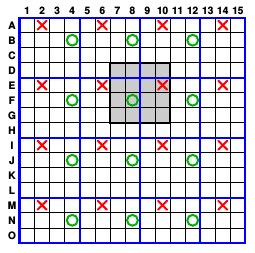
\includegraphics[width=0.6\textwidth]{work_dist_strategy.png}
  \caption{The uv grid is divided into smaller subgrids, each the size of the the support region of the precomputed convolution function. Each thread monitors a single
  grid cell at a time. Therefore a single thread will be monitoring the highlighted position marked by the cross and another marked by the circle. The highlighted block of 
  threads moves only when the central uv-coordinate is gridded to a new grid cell. At that point the accumulated register values are written to global memory using atomic 
  operations. Image taken from Romain \cite{romein2012efficient}.}
  \label{IMG_WORK_DIST_STRATEGY}
 \end{mdframed}
\end{figure}

Previous work on GPU acceleration has focussed solely on implementing uv-space w-projection and its associated w-dependent convolution functions. However, the GPU gridding 
operation remains essentially the same and will form the basis of our own work on GPU-based faceted imaging.

\section{Work plan}
A brief schedule is given below:\\
\begin{tabular}{|p{2.5cm}|p{5cm}|}
 \hline
 \textbf{Due} & \textbf{Task} \\
 \hline
 30 June 2014 & Prototype of faceted gridder, introduction and background chapters\\
 \hline
 31 August 2014 & C++ CPU Implementation\\
 \hline
 31 October 2014 & GPU Implementation\\
 \hline
 7 January 2015 & Optimized GPU Implementation\\
 \hline
 30 March 2015 & MPI implementations and design chapter\\
 \hline
 31 July 2015 & Possible experimentation with hybrid faceted w-projection\\
 \hline
 31 August 2015 & Results and analysis chapter\\
 \hline
 31 October 2015 & Final draft corrections \\
 \hline
\end{tabular}
{
{\footnotesize \bibliography{proposal}}
\bibliographystyle{plain}
}
\end{document}
